\begin{abstract}
	En el año 2020 los casos detectados de cáncer de mama en Colombia fueron 15.509 de los cuales 4.411 terminaron en muerte \cite{InternationalAgencyforResearchonCancer2020}. El pronóstico anticipado de esta enfermedad se ha convertido en una necesidad de investigación debido a que puede facilitar el tratamiento preventivo para evitar su letalidad en un estado avanzado. Esta investigación se centra esencialmente en la aplicación de la minería de datos para diagnosticar y caracterizar la morbilidad por cáncer de mama  en la ciudad de Pereira-Risaralda según la edad, el genero, la zona y el tipo de régimen de salud.
\end{abstract}

\section{INTRODUCCIÓN }

El Municipio de Pereira perteneciente al departamento de Risaralda, se localiza en el centro-occidente del territorio colombiano, en un pequeño valle formado por la terminación de un contra fuerte que se desprende de la Cordillera Central y estratégicamente como parte del abanico central del país dentro de la región cafetera \cite{Pereira2002}. La Secretaría de Salud departamental de este municipio en 2021 dio conocer las cifras de afectación por cáncer de mama, en donde se detecto que esta enfermedad cobra la vida de 17 risaraldenses por 100 mil habitantes, ubicando al departamento en el décimo lugar a nivel nacional por mortalidad de dicha enfermedad oncológica \cite{Risaralda2021}. El pronóstico anticipado de este tipo de cáncer en el municipio de Pereira se convirtió en una necesidad de investigación, ya que puede facilitar el tratamiento preventivo para evitar su letalidad en un estado avanzado. La minería de datos ha sido utilizada por diversos investigadores para modelar la progresión y el tratamiento de afecciones cancerosas debido a su capacidad para detectar características significativas en conjuntos de datos complejos, dado lo anterior el proposito de esta investigación es generar un diagnóstico significativo de la probabilidad que tiene una muestra de la población risaraldense de padecer cáncer de mama según su edad, genero, zona  y régimen de salud, esto con el proposito priorizar el tratamiento oncológico y así ayudar a disminuir la morbilidad por cáncer este municipio.


\section{PROBLEMA DE ESTUDIO}
Pereira cuenta con una población estimada de 477.027 habitantes de los cuales 399.283 están ubicados en el área urbana y 77.744 en el área rural \cite{DANE2021}. Este municipio presentó para el año 2019 un total 363 de casos nuevos y 8 decesos de cáncer de mama. Estos casos aumentaron en el año 2020, registrando 278 casos nuevos y 5 fallecimientos. Para el año 2021 se tuvieron más de 260 casos con una incidencia de la enfermedad de 36 casos nuevos y 17 casos de muerte por cada 100 mil habitantes risaraldenses \cite{Risaralda2021}.

Colombia presenta limitaciones con respecto al acceso de la detección y el diagnóstico temprano del cáncer, provocado en la mayoría de los casos por factores como el estrato socio-económico, la cobertura del seguro de salud, el origen y la accesibilidad. En promedio, el tiempo de espera de un paciente es de 90 días desde la aparición de los síntomas hasta el diagnóstico de dicho cáncer. La primera acción para reducir la tasa de mortalidad por cáncer de mama debe estar enfocada en la agilidad del diagnóstico y el acceso oportuno a la atención\cite{Duarte2021}. 

Aunque un diagnóstico a tiempo es la clave en la lucha contra el cáncer de mama, más de un 30\% de las colombianas lo detectan cuando la enfermedad está muy avanzada. Lo anterior aumenta el riesgo de morir y disminuye la respuesta favorable al tratamiento de este tipo de cáncer \cite{Risaralda2021}. Dado el aumento de casos nuevos y número de muertes año tras año en este municipio, es imprescindible realizar el diagnostico anticipado de esta enfermedad para facilitar el tratamiento preventivo y así evitar que este tipo de cáncer sea inmanejable en un estado avanzado. Una alternativa para disminuir la tasa de mortalidad es predecir e identificar, con base al análisis de un conjunto de datos, que probabilidad tiene un individuo de contraer el cáncer de mama según la edad, el genero, zona y el tipo de régimen de salud ,esto con el propósito de priorizar el tratamiento oncológico a través de cirugías, radiación, medicamentos y otras terapias para detener la progresión de esta enfermedad y así disminuir la morbilidad en este municipio.

Considerando que la minería de datos es un campo multidisciplinario que utiliza uno o varios algoritmos con el fin de identificar tendencias y patrones interesantes dentro de los datos, es la mejor opción para generar un diagnóstico significativo de la probabilidad que tiene una muestra de la población de Risaralda de padecer de cáncer de mama. La  minería de datos es de gran utilidad para la exploración de patrones ocultos en las bases de datos del ámbito médico. Estos patrones se utilizan ampliamente en el campo del diagnóstico clínico debido a que los datos médicos originales son de naturaleza heterogénea, voluminosa y distribuida \cite{Nalinipriya2021}.

Así, el objetivo de esta investigación es aplicar las etapas de la metodología KDD\footnote{Knowledge Discovery in Databases} al conjunto de datos de morbilidad por cáncer entre los años 2019 y 2021 en el municipio de Pereira-Risaralda. Esto con la finalidad de pronosticar y caracterizar el tipo de población mas susceptible de padecer esta enfermedad según su edad, genero, zona y régimen de salud.

\section{APLICACIONES DE ALGORITMOS ML Y DL EN EL DIAGNOSTICO DEL CÁNCER DE MAMA}
Diversas técnicas de ML\footnote{Machine Learning} y DL\footnote{Deep Learning} aplicadas en el diagnóstico del cáncer de mama han sido propuestas por una gran cantidad de investigadores.Las siguientes investigaciones fueron seleccionadas por su relevancia y aporte para el diagnostico del cáncer de mama debido a que brindan una gran cantidad de información y son un punto de partida importante para aplicar el proceso de minería de datos con dicho fin. Las investigaciones seleccionadas como referentes a nivel de modelos se muestran a continuación:

\cite{Alakwaa2018} realizaron la identificación de subtipos moleculares sobre datos metabolómicos por medio de algoritmos de DL y ML para determinar el pronóstico del cáncer de mama y la selección terapéutica. Para ello, la investigación se basa en la clasificación de dicho cáncer en cuatro subtipos moleculares: Luminal A ($ER +, PR \pm$ y $HER2-$), Luminal B ($ER +, PR \pm,$ y $HER2\pm$), $HER2-$ enriquecido ($ER-, PR-$ y $HER2 +$) y triple negativo ($ER-, PR-$ y $HER2 -$). Estos subtipos son generados a partir de las proteínas de factor de crecimiento epidérmico receptor 2 (HER2), receptor de progesterona (PR) y receptor de estrógeno (ER) encargadas de estimular el crecimiento y la diferenciación celular. Los resultados de supervivencia difieren significativamente entre estos subtipos. Los subtipos luminales A y B tienen un pronóstico benigno sin embargo, los tumores triple negativos y los tumores $HER2$ tienen un pronóstico maligno. Para la investigación se utilizó un data-set conformado por 271 muestras de cáncer de mama ($204$ $ER+ $ y $67$ $ER- $) del Departamento de Patología del Hospital Charité. Posterior a eso para complementar dicho data-set se midieron un total de 162 metabolitos con estructura química conocida mediante cromatografía de gases para todas las muestras de tejido. Para realizar la clasificación de los datos metabólicos obtenidos se utilizó una Red Neuronal FNN\footnote{Feedforward Neural Network} y los siguientes modelos de ML: RF, SVM, RPART\footnote{Recursive Partitioning}, LDA\footnote{Linear Discriminant Analysis}, PAM\footnote{Microarray Prediction Analysis} y GBM\footnote{Gradient Boosting Machine}. Posteriormente, se realizó una validación cruzada (Cross-validation) con el 80\% de los datos de entrenamiento y se probaron los modelos con el 20\% de los datos restantes. Para finalizar, se utilizaron las medidas AUC\footnote{Area Down The Curve} y ROC\footnote{Receiver Operating Characteristic Curve} para evaluar el rendimiento general de los dichos modelos. En conclusión, esta investigación determino que las FNN muestran una precisión de predicción (AUC = $0,93$) mayor sobre los métodos de ML al realizar la clasificación del cáncer de mama en los subtipos moleculares basados en el receptor de estrógeno(ER).

\cite{Nateghi2021} proponen de un sistema basado en métodos de DL y ML para la predicción de la proliferación tumoral a partir de imágenes WSI \footnote{ Whole Slide Images } obtenidas del recuento mitótico. La proliferación tumoral, que se correlaciona con el grado del tumor, es un biomarcador crucial que indica el pronóstico de las pacientes con cáncer de mama. El método más utilizado para predecir la velocidad de proliferación tumoral es el recuento de figuras mitóticas en los portaobjetos histológicos de hematoxilina y eosina ($H\&E$). El recuento manual de mitosis consiste en identificar células tumorales implicadas en el proceso anormal de la división celular. Para la investigación se utilizó el data-set proporcionado por el desafío de evaluación de la proliferación tumoral (TUPAC16) en donde el objetivo es evaluar algoritmos que predicen las puntuaciones de proliferación tumoral a partir de imágenes WSI. Primero, al considerar el tejido epitelial como regiones de actividad de mitosis, los investigadores propusieron un método de detección de regiones de interés basado en DL para seleccionar las regiones de alta actividad de mitosis a partir de las imágenes proporcionadas en el desafío. Posteriormente, se entrenó un conjunto de redes neuronales para detectar la propagación de la mitosis en distintas áreas seleccionadas. Para finalizar, los investigadores entrenaron el modelo SVM para predecir la puntuación final de proliferación tumoral. La precisión del algoritmo entrenado logró una medida-F del 73,81\% y un coeficiente kappa ponderado de 0,612, respectivamente, superando significativamente otros algoritmos que participaron en el desafío TUPAC16. Como conclusión de la investigación, los resultados experimentales demuestran que el algoritmo propuesto basado en el paradigma de DL y ML mejoró considerablemente la precisión de la predicción de la proliferación tumoral y proporciono un modelo con una precisión confiable para respaldar la toma de decisiones a nivel médico.

\cite{McKinney2020} desarrollaron un modelo de DL para identificar el padecimiento del cáncer de mama mediante imágenes mamográficas obtenidas en el Reino Unido y EE. UU. La mamografía tiene como objetivo identificar el cáncer de mama en las primeras etapas de la enfermedad, cuando el tratamiento puede tener más éxito. A pesar de la existencia de diversas técnicas de detección del cancér de mama en todo el mundo, la interpretación de las mamografías se ve afectada por altas tasas de falsos positivos y falsos negativos. El data-set del Reino Unido consistió en mamografías recopiladas de 25,856 mujeres entre 2012 y 2015 en dos centros médicos en Inglaterra, donde las mujeres se examinan cada tres años. Incluyó a 785 mujeres a las que se les realizó una biopsia y a 414 mujeres con una diagnóstico maligno del cáncer dentro de los 39 meses posteriores a la obtención de imágenes. El data-set de EE. UU consistió en mamografías que se recolectaron entre 2001 y 2018 de 3.097 mujeres en un centro médico académico. Se incluyeron imágenes de las 1511 mujeres a las que se les realizó una biopsia durante este período de tiempo y de un subconjunto aleatorio de mujeres que nunca se sometieron a una biopsia. Entre las mujeres que recibieron una biopsia, 686 fueron diagnosticadas con cáncer dentro de los 27 meses posteriores a la obtención de las imágenes. Los casos que fueron diagnosticados como positivos para cáncer fueron acompañados de un diagnóstico confirmado por biopsia dentro del período de seguimiento. una reducción absoluta del 5,7\% y 1,2\% (EE.UU. Y Reino Unido) en falsos positivos y del 9,4\% y 2,7\% en falsos negativos. En la investigación los data-set obtenidos no se utilizaron para entrenar ni ajustar el modelo basado IA. Como resultados, la investigación proporciono evidencia de la capacidad del modelo basado en IA y DL para generalizarse desde el Reino Unido a los EE.UU. En un estudio independiente de seis radiólogos, el sistema de IA superó el diagnóstico obtenido por dichos radiólogos con una precisión (AUC-ROC) mayor que la generada por el radiólogo promedio. Además, para comprobar la predicción del modelo los investigadores realizaron una simulación en la que el sistema de IA participó en el proceso de doble lectura de diagnóstico que se utiliza en el Reino Unido y se descubrió que el sistema de IA mantuvo un rendimiento elevado y redujo la carga de trabajo del segundo lector en un 88\%. Como conclusión, esta investigación demostró que las técnicas de IA mejoran la precisión y la eficiencia de las técnicas tradicionales para la detección del cáncer de mama.


\cite{Mullooly2019} utilizaron técnicas de DL para identificar correlaciones histológicas en biopsias de la densidad mamaria obtenidas por técnicas radiológicas para determinar el cáncer de mama entre mujeres con una densidad del tejido fibroglandular alto o bajo. La densidad de la mama es una característica radiológica que refleja el contenido de tejido fibroglandular en relación con el área o el volumen de la mama y es considerada como un factor de riesgo de padecer cáncer. En la investigación se evaluaron imágenes digitalizadas teñidas con hematoxilina y eosina ($H\&E$) de biopsias de 852 pacientes. La densidad mamaria se evaluó como volumen fibroglandular global y localizado. Posteriormente, los investigadores modelaron una Red Neuronal CNN para caracterizar la composición de $H\&E$. En total, se extrajeron 37 características de la salida de la red, que describen las cantidades de tejido y la estructura morfológica. Se entrenó un modelo de regresión por Bosque Aleatorio (RF) para identificar correlaciones predictivas del volumen fibroglandular en 588 pacientes. Se evaluaron las correlaciones entre el volumen fibroglandular predicho y cuantificado radiológicamente en 264 pacientes independientes. Se entrenó un segundo clasificador de bosque aleatorio (RF) para predecir el diagnóstico invasivo vs. el diagnóstico benigno; el rendimiento de los algoritmos se evaluó utilizando el área bajo la curva (AUC). Utilizando características extraídas, los modelos de regresión predijeron el volumen fibroglandular global con una precisión de 0,94 y localizado con una precisión de 0,93 teniendo como base el contenido del estroma graso y no graso representando las correlaciones más fuertes seguidas de la cantidad de tejido epitelial. Para predecir el cáncer entre el volumen fibroglandular elevado y bajo, el clasificador logró un valor AUC de 0,92 y 0,84, respectivamente, siendo las características de tejido epitelial las más importantes. Estos resultados sugieren que el estroma no graso, la cantidad de tejido graso y el tejido epitelial predicen el volumen fibroglandular. Como conclusión, la investigación demostró que los modelos de DL y ML permiten identificar correlaciones histológicas con riesgo de cáncer en pacientes con alta y baja densidad de tejido fibroglandular.

\cite{Hu2020} desarrollaron una técnica para el diagnóstico asistido por computadora CAD\footnote{Computer-Aided Diagnosis} bajo el paradigma de aprendizaje por transferencia profunda para realizar la diagnosis del cáncer de mama utilizando mpMRI\footnote{Multiparametric Magnetic Resonance Imaging}.El estudio incluyó imágenes clínicas de resonancia magnética de 927 lesiones únicas de 616 mujeres, en donde se excluyeron las imágenes de lesiones que no presentaban una lesión visible, lesiones que no tenían validación de diagnóstico final, o lesiones que no pudieron ser claramente asignadas en a la categoría benigna ni maligna. Cada estudio de resonancia magnética RM\footnote{Magnetic Resonance}, incluyó una secuencia con contraste dinámico DCE\footnote{Dynamic Contrast-Enhanced} y una imagen de RM ponderada en un radio T2w\footnote{T2 weighted image}. Se utilizó una Red Neuronal CNN previamente entrenada para extraer características de las imágenes DCE y T2w, y se entrenaron modelos SVM en las características de CNN para distinguir entre lesiones benignas y malignas. La información de las imágenes de resonancia magnética con contraste dinámico (DCE) y ponderada en T2w se añadió al modelo IA de tres formas diferentes: fusión de imágenes, fusión de características y fusión de clasificadores. La fusión de imágenes, se utilizó para crear una imagen compuesta RGB con base a las imágenes DCE y T2w. La fusión de características, para combinar las características generadas por las redes neuronales convolucionales con base a las imágenes DCE y T2w para posteriormente ser utilizadas como entrada en un algoritmo de máquina de vectores de soporte (SVM). La fusión clasificadora se utilizó para calcular la probabilidad de malignidad por medio de voto suave (soft-voting) con base al resultado obtenido por el algoritmo SVM al analizar las imágenes DCE y T2w. El rendimiento de los modelos de DL se evaluó utilizando la curva (ROC) y fue comparado utilizando la prueba DeLong. El método de fusión de características superó estadísticamente de manera significativa a los demás métodos. En conclusión, el método propuesto de aprendizaje de transferencia profunda CAD para mpMRI pudo mejorar el diagnóstico del cáncer de mama al reducir la tasa de falsos positivos y mejorar el valor predictivo positivo en la interpretación de imágenes obtenidas por resonancia magnética.

\cite{Shia2021}, propusieron  un método de ML y diseño de una metodología para el análisis de la clasificación de tumores de mama benignos y malignos en imágenes de ultrasonido sin necesidad de un procesamiento de selección regional tumoral a priori.  Las imágenes se recopilaron desde el 1 de enero de 2017 hasta el 31 de diciembre de 2018. En total, se examinaron 370 masas benignas y 418 malignas, y se estudiaron a 677 pacientes en este estudio. Los criterios de exclusión para pacientes con tumores benignos incluyeron tipos de tejido que se asociaron con las siguientes afecciones: inflamación (incluida la autoinflamación, inflamación crónica e inflamación xantogranulomatosa), abscesos y dermatitis espongiótica. Para los pacientes con tumores malignos, los criterios de exclusión incluyeron casos con tipos de tejido incompletos, clasificación de categoría BI-RADS\footnote{Breast Imaging Reporting and Data System} desconocida o informes de imágenes incompletas. Las edades de los pacientes oscilaron entre los 35 y los 75 años.  El data-set recopilado constaba de 677 imágenes (Benignas: 312, maligno: 365) obtenidas de diferentes centros oncológicos de Estados Unidos. Una vez generado el data-set de estudio se procedió a realizar la extracción de características de las imágenes a través del método de histograma de gradientes orientados HOG\footnote{Histogram of Oriente Gradients} y el método histograma piramidal de gradientes orientados PHOG\footnote{Pyramid Histogram of Orientad Gradients}. Adicionalmente, se utilizó el método FAST\footnote{Features from the Accelerated Segment Test} para determinar si se podían extraer características de clasificación importantes de las imágenes preliminares. El HOG se utilizó para extraer información útil y descartar información redundante para simplificar la clasificación de imágenes calculando y contando histogramas de gradiente de áreas específicas. La distancia entre dos descriptores de imágenes PHOG refleja la medida en que las imágenes contienen formas similares y corresponde a sus diseños espaciales y el método FAST permite un rendimiento mayor que otros métodos en la detección de esquinas de los mamogramas para extraer puntos característicos y luego rastrear y mapear objetos con características relevantes en dichas imágenes. El siguiente paso fue realizar la selección de características por medio de la técnica de selección de características basada en correlación CFS\footnote{Correlation Based Feature Selection} para evaluar los atributos importantes, y crear un subconjunto de datos considerando las habilidades predictivas junto con el grado de redundancia. La función de evaluación se utilizó para evaluar subconjuntos que contenían características que estaban altamente correlacionadas con la clase y no estaban correlacionadas entre sí. Se ignoraron las características irrelevantes y se excluyeron las características redundantes. Finalmente, se realizó la clasificación de características con base en la combinación de aprendizaje ponderado localmente LWL\footnote{Local Weighted Learning }, la optimización secuencial mínima SMO\footnote{Sequential Minimal Optimization} y el  método KNN.  Para la evaluación del desempeño de la clasificación, se utilizó la técnica de validación cruzada para determinar el porcentaje de error, la media, la desviación estándar y el intervalo de confianza para los algoritmos de referencia.  La precisión diagnóstica se estimó comparando las curvas AUC y ROC con la prueba no paramétrica de DeLong. El rendimiento de clasificación del conjunto de datos de imágenes mostró una sensibilidad del 81,64\% y una especificidad del 87,76\% para imágenes malignas con AUC de 0,847. Los valores predictivos positivos y negativos fueron 84,1 y 85,8\%, respectivamente. En conclusión, la comparación de los diagnósticos médicos y el diagnóstico generado por el modelo de ML propuesto arrojó resultados similares. Esto indica la posible aplicabilidad del ML en la generación de diagnósticos clínicos.

\cite{Shen2019} desarrollaron un algoritmo de DL que puede detectar con precisión el cáncer de mama en mamografías usando un entrenamiento e2e \footnote{end-to-end} que aprovecha de manera eficiente los data-sets de imágenes mamográficas obtenidas a través de diagnósticos asistidos por ordenador CAD . En este enfoque las anotaciones para identificación de lesiones en la mama obtenidas de las imágenes mamográficas solo se utilizaron en la etapa de entrenamiento inicial, y las etapas posteriores requirieron solo las características obtenidas a nivel de imagen, eliminando la dependencia de diagnósticos obtenidos de estas anotaciones. El algoritmo generado fue testeado con dos data-set de prueba. El primer data-set fue obtenido de la base de datos de mamografías digitales del sitio web CBIS-DDSM. Este data-set almacenaba 2478 imágenes de mamografías de 1249 mujeres e incluía vistas tanto craneocaudales (CC) como oblicuas mediolaterales (MLO), además contaba con etiquetas confirmadas patológicamente en una categoría benigna o maligna para la mayoría de los exámenes. Con este data-set, el modelo logró una predicción con un valor AUC de 0,88 y el promedio de cuatro modelos entrenados posteriormente mejoró esta predicción a valor AUC de 0,91 con una sensibilidad de 86,1\% y especificidad de 80,1\%. El segundo data-set fue obtenido de la base de datos de mamografías digitales INbreast FFDM\footnote{Full-Field Digital Mammography} la cual contenía información de 115 pacientes y 410 mamografías, este data-set también incluía vistas CC y MLO. Con el segundo data-set el modelo logró una predicción con valor AUC de 0,95, y el promedio de cuatro modelos entrenados mejoró el AUC a 0,98 con una sensibilidad de 86,7\% y especificidad de 96,1\%. La investigación demostró que el entrenamiento generado en una Red Neuronal CCN con el enfoque e2e CBIS-DDSM se puede transferir a imágenes FFDM de INbreast utilizando solo un subconjunto de datos para ajustar el modelo y sin depender de la disponibilidad de anotaciones de lesiones. Estos hallazgos demostraron que los métodos de DL se pueden utilizar para lograr una alta precisión de diagnosis en mamografía heterogéneas y es muy prometedor para mejorar las herramientas clínicas para reducir la detección de falsos positivos y falsos negativos de cáncer de mama.

\cite{Naik2020} utilizaron el paradigma de DL con base al diagnóstico del cáncer de mama a partir del estado molecular del receptor de Estrógeno ERS\footnote{Estrogen Receptor Status},determinado por los patólogos a partir de la tinción inmunohistoquímica IHC\footnote{Inspection Immunohistochemistry} que destaca la presencia de antígenos de superficie celular del tejido obtenido a través de una biopsia. Para lograrlo, se recopilaron imágenes WSI teñidas con hematoxilina y eosina (H\&E) del data-set obtenido del Banco Australiano de tejidos para el cáncer de mama ABCTB\footnote{Australian Breast cáncer Tissue Bank}, que contenía 2535 imágenes de exámenes realizados  a pacientes y el data-set obtenido del Atlas genómico del cáncer TCGA\footnote{The Cancer Genomic Atlas}, que contenía 1014 imágenes de 939 pacientes. Ambos conjuntos de datos informaban el estado de la presencia de receptor de Estrógeno (ER), receptor de Progesterona (PR) y el de factor de crecimiento epidérmico receptor 2 (HER2) determinado por patólogos encargados de la inspección visual de los portaobjetos teñidos mediante IHC. Los WSI se escanearon a una resolución de 20x o superior. Posteriormente, se utilizó el modelo de aprendizaje de instancias múltiples MIL\footnote{Multiple Instance Learning}, el cual fue entrenado usando tinciones H\&S y anotaciones IHC como etiquetas de datos de entrada. El modelo MIL se utilizó para estimar el ERS a partir de mosaicos seleccionados al azar de un WSI. Para lograr la interpretabilidad al localizar mosaicos discriminativos en imágenes de H\&E e identificar características histomorfológicas que se correlacionan con el crecimiento celular impulsado por hormonas, los investigadores diseñaron una arquitectura bajo el paradigma de redes neuronales profundas llamada \textit{ReceptorNet} basada en el proceso ejecutado por el modelo MIL. ReceptorNet aprende a asignar altos pesos a los mosaicos en la imagen de H\&E que tienen la máxima capacidad discriminativa, y a asignar bajos pesos a los mosaicos que son insignificantes para el proceso de aprendizaje y diagnóstico. El análisis de los pesos asignados permitió determinar los mosaicos que se utilizaron para realizar la estimación de ERS.  La arquitectura de ReceptorNet consta de tres redes neuronales interconectadas: un módulo extractor de funciones, un módulo de aprendizaje y un módulo de decisión. Adicionalmente, se comparó el método propuesto con dos métodos MIL ampliamente utilizados: Meanpool y Maxpool. En Meanpool, las representaciones de características de mosaicos se promedian para obtener una representación de características agregadas. En Maxpool, se obtiene un máximo de características para cada una de las dimensiones de características. Estos métodos se entrenaron en la misma arquitectura de modelo que ReceptorNet. El algoritmo propuesto logro una curva AUC de sensibilidad y especificidad de 0,92. En conclusión, esta investigación demostró una estimación precisa del estado del receptor de ER a partir de tinciones de H\&E utilizando una Red Neuronal lo cual impacta en la disminución del trabajo al realizar procesos patológicos. En términos más generales, el estudio represento una mejora de los métodos médicos para el diagnóstico del cáncer de mama y demostró el potencial del ML para mejorar el pronóstico y diagnóstico del cáncer mediante el aprovechamiento de señales biológicas imperceptibles para el ojo humano.

\cite{Roszkowiak2021} proponen el modelo CHISEL\footnote{Computer assisted Histopathological Image Segmentation and Evaluation} para Segmentación y evaluación de imágenes histopatológicas asistidas por computadora. Este sistema e2e es capaz de evaluar cuantitativamente muestras digitales (benignas y malignas) con tinción nuclear inmunohistoquímica IHC de diversa intensidad y compacidad del tejido afectado por el cáncer de mama. El modelo fue capaz de procesar imágenes patológicas digitales, núcleos de microarrays de tejido TMA\footnote{Tissue Micro Array} y muestras adquiridas por cámara digital conectada a un microscopio. Una de las características principales de CHISEL es la segmentación de imágenes con base a regiones de interés ROIs\footnote{Regions of Interest}. El data-set utilizado fue recopilado con base a imágenes de tejido de cáncer de mama adquiridas de diversas universidades, laboratorios, hospitales y departamentos de patología ubicados en España. Las secciones de tejido de las biopsias de mama y ganglios auxiliares se sometieron a un procesamiento histotécnico tradicional y se convirtieron en bloques de tejido embebidos en parafina y fijados con formalina. Los TMA se formaron extrayendo pequeños cilindros de tejido colocados en una matriz en un bloque de parafina. Posteriormente, se tiñeron con los anticuerpos primarios IHC indirectos contra FOXP3\footnote{proteína P3 de la Forkhead box} y los anticuerpos secundarios, incluido el bloque de peroxidasa, polímero marcado, tamponado con sustrato cromógeno DAB+ y finalmente contrastado con hematoxilina. La tinción simultánea de múltiples muestras en TMA disminuye la variabilidad intralaboratorio de la diferencia en las concentraciones de tinción entre cortes. El TMA tiene una gran ventaja para procesar imágenes digitales porque se adquieren múltiples muestras en un escaneo bajo las mismas condiciones. En general, el uso de TMA aumenta la reproducibilidad de los estudios de patrones de biomarcadores. El modelo propuesto se centró en procesar las imágenes teñidas con IHC (especialmente DAB \& H) para posteriormente estimar la masa de células beta y el número de núcleos dentro del área teñida de insulina. El data-set estaba conformado por 20 imágenes de muestras de tejido teñidas con DAB y H. El modelo utilizo el paradigma de ML y el procesamiento local recursivo para eliminar los contornos distorsionados (inexactos) del conjunto de datos adquiridos. El método se validó utilizando dos data-set etiquetados que demostraron la relevancia de los resultados obtenidos. La evaluación se basó en el conjunto de datos IISPV de tejido de biopsia de pacientes con cáncer de mama, con marcadores de células T, junto con el conjunto de datos Warwick BetaCell de tejido teñido con DAB y H de pacientes con diabetes post-mórtem. Posteriormente, se utilizaron Redes neuronales Artificiales ANN\footnote{Artificial Neural Network} para clasificar las imágenes en categorías malignas o benignas, y se optimizó el algoritmo analizando la influencia del número de capas, el número de neuronas y las funciones de activación en los resultados de la clasificación. Finalmente, la clasificación dio como resultado una precisión media del 99,2\% que se probó con cinco validaciones cruzadas. Este modelo resuelve el complejo problema de la cuantificación de núcleos en imágenes digitalizadas de cortes de tejido teñidos inmunohistoquímicamente, logrando los mejores resultados para muestras de tejido de cáncer de mama teñidas con DAB y H. Para facilidad de manejo del modelo, se generó una interfaz gráfica (GUI) y se optimizó para utilizar completamente la potencia informática disponible. Con base a los resultados de los objetos detectados y clasificados con base a algoritmos de DL y ML, se llegó a la conclusión de que el método propuesto puede lograr resultados mejores o similares a los métodos de última generación. 

\cite{Negahbani2021} propusieron un conjunto de datos denominado SHIDC-BC-Ki-67 basado en la proteína nuclear Ki-67 y los linfocitos infiltrantes de tumores TIL \footnote{Tumor Infiltrating Lymphocytes},los cuales son factores determinantes para predecir la progresión de un tumor cancerígeno y  la respuesta probable del mismo a la quimioterapia. Teniendo en cuenta que la estimación de ambos factores depende de la observación de patólogos profesionales y que también pueden existir variaciones interindividuales, los métodos automatizados que utilizan algortimos de ML, específicamente los enfoques basados en el DL, son llamativos para realizar el diagnóstico y pronóstico del cáncer de mama. Sin embargo, los modelos de DL necesitan una cantidad considerable de datos etiquetados y este fue el motivo por lo cual se propuso la creación del data-set SHIDC-BC-Ki-67. Adicionalmente, en la investigación realizada se presenta una arquitectura en pipeline, para la estimación de la proteína Ki-67 y la determinación simultánea de la puntación de TIL intratumoral en células cancerígenas. El data-set recopilado estaba formado por imágenes digitales de muestras microscópicas con tinción nuclear inmunohistoquímica IHC obtenidas a través de biopsias realizadas con aguja gruesa(CNB) de tumores de mama malignos del tipo de carcinoma ductal invasivo. Además, se usó hematoxilina para realizar la tinción nuclear y semicuantificar el grado de inmunotinción. Las muestras de la biopsia fueron recolectadas durante un estudio clínico de 2017 a 2020. El data-set SHIDC-B-Ki-67 contiene 1656 datos de entrenamiento y 701 de prueba. Todos los pacientes que participaron en este estudio eran pacientes con un diagnóstico patológicamente confirmado de cáncer de mama cuyas biopsias fueron tomadas en los laboratorios de patología de los hospitales afiliados a la Universidad de Ciencias Médicas de Shiraz en Shiraz, Irán. Para la adquisición de las imágenes se realizaron los siguientes pasos: Primero, el patólogo identifica el tumor y define una región de interés ROI. Para cubrir todo el ROI, se capturan varias imágenes que pueden superponerse. El patólogo selecciona preferentemente imágenes del área tumoral. Luego, patólogos expertos etiquetaron las imágenes teñidas como células tumorales positivas y negativas para Ki-67 y células tumorales con linfocitos infiltrantes positivos. Finalmente, se realizó la clasificación celular y la detección de Ki-67 y TIL, para lograrlo, se usaron Redes Neuronales Convergentes(CNN) para extraer características relevantes y estimar mapas de densidad a partir de una imagen RGB\footnote{Red, Green, Blue} de entrada. PathoNet primero extrae características de las imágenes de entrada y luego predice los píxeles candidatos para las células inmuno-positivas e inmuno-negativas Ki-67, y también los linfocitos con sus valores de densidad correspondientes. El backend propuesto utiliza capas convolucionales para la detección, clasificación y recuento de células en imágenes histopatológicas. Posteriormente se utilizo el algoritmo de Watershed para asignar imágenes en escala de grises a un espacio de relieve topográfico. La arquitectura en pipeline propuesta estaba conformada de una red PathoNet, posprocesamiento y el algoritmo de Watershed. En conclusión, en esta investigación se propuso un nuevo punto de referencia para la detección celular, la clasificación, la estimación del índice de proliferación y la puntuación de TIL mediante imágenes histopatológicas procesadas con modelos de DL para la extracción de características que permiten generar un data-set para la estimación intratumoral en células de cáncer de mama.


\section{METODOLOGÍA}

{\tiny }La minería de datos tiene su origen en las áreas de estadística, matemáticas, aprendizaje automático e inteligencia artificial. El término apareció por primera vez en la comunidad académica hacia 1995. La expresión \textit{Descubrimiento de conocimientos en bases de datos} (KDD) se acuñó en 1989 para subrayar que el conocimiento puede derivarse del descubrimiento basado en datos. Técnicamente, el KDD es la aplicación del método científico a la minería de datos. Además, un modelo de proceso KDD típico incluye una metodología para la extracción y preparación de los datos, así como la toma de decisiones sobre las acciones que deben realizarse una vez que se ha realizado la minería \cite{Roiger2017}.  

En la presente investigación, se adoptó las fases consecutivas del método KDD \cite{Shafique2014} para el descubrimiento de conocimiento y posterior toma de decisiones, teniendo como base el conjunto de datos de Morbilidad por cáncer de mama en el municipio de Pereira-Risaralda entre los años 2019 y 2021.

\subsection{Fase 1: Comprender el dominio de la aplicación}
En esta etapa se definieron los objetivos y el dominio de la aplicación, este caso tenemos que:

\begin{itemize}[label=\HandRight]
	\item \textit{\textbf{Dominio:}} Ciencias de la salud y protección social enfocada en los casos cáncer de mama presentados en la población del municipio de Pereira ubicado en el Departamento de Risaralda en Colombia.\\
	\item \textit{\textbf{Objetivo:}} Aplicar las etapas de la metodología KDD al conjunto de datos de morbilidad por cáncer en el municipio de Pereira-Risaralda.\\
	\item \textit{\textbf{Pregunta:}} ¿Presenta el cáncer de mama indices mas altos de muertes en muestras de la población de Pereira-Risaralda caracterizada según su edad, genero, zona y régimen de salud ?
\end{itemize}

\newpage
\subsection{Fase 2: Selección de datos}
En esta etapa se obtuvo el un conjunto de datos de \textit{Morbilidad por cáncer en Pereira} entre los años 2019 y 2021. Cabe resaltar, que los datos fueron solicitados a la secretaria de salud de la alcaldía Municipal de Pereira por medio de la pagina \textit{https://www.datos.gov.co/}. Este conjunto de datos consta de un tamaño de $40.658$ filas y $7$ columnas: 
\begin{itemize}[label=\SquareShadowTopLeft]
	\item  \textit{\textbf{NOMBRE DIAGNOSTICO:}} 	
	Nombre de la enfermedad.
	\item  \textit{\textbf{CÓDIGO DIAGNOSTICO:}} 	
	Códigos únicos de procedimientos en salud, código que identifica el diagnostico.
	\item  \textit{\textbf{EDAD:}} 	
	Edad del paciente.
	\item  \textit{\textbf{SEXO:}} 	
	Sexo del paciente.
	\item  \textit{\textbf{ZONA:}} 	
	Zona rural o urbana donde vive el paciente.
	\item  \textit{\textbf{RÉGIMEN:}} 	
	Tipo de vinculación de la persona al sistema general de salud .
	\item  \textit{\textbf{AÑO:}} 	
	Año en que se realiza el diagnostico.
\end{itemize}

A continuación, se realizó un \textit{Análisis exploratorio de datos} para descubrir patrones generales en el conjunto de datos propuesto. En primer lugar, se determino que el código $C509$, relacionado a un tumor maligno de la mama con una localización no especificada, es el mas tipo de cáncer mas frecuente de la totalidad del conjunto de datos, para lograrlo se utilizó la representación gráfica de nube de palabras que se muestra en la figura \ref{WORD_CLOUD}.

\begin{figure}[h!]
	\centering
	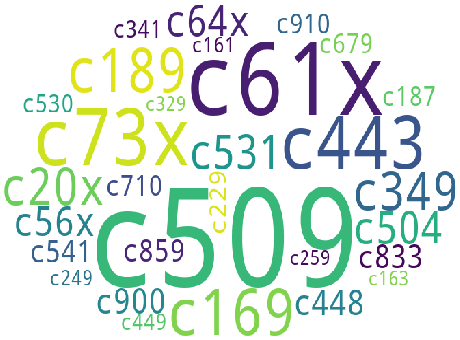
\includegraphics[width=0.84
	\linewidth]{IMAGENES/WORD_CLOUD}
	\caption{Nube de palabras con los tipos de cáncer frecuentes.}
	\label{WORD_CLOUD}
\end{figure}

Dadas las variables anteriores, se seleccionaron aquellos registros de los pacientes que fallecieron por tumores producidos por cáncer de mama según el manual de codificación y estadificación del programa de Vigilancia, Epidemiología y Resultados Finales \textit{SEER} \footnote{SEER: Surveillance, Epidemiology, and End Results}. Cabe resaltar, que este programa brinda información sobre las estadísticas del cáncer en un esfuerzo por reducir la morbilidad causada por esta enfermedad en Estados Unidos \cite{SEER2022}. El filtrado de los registros fue realizado a través de la variable \textit{CÓDIGO DIAGNOSTICO} según los códigos topográficos del $C500$ al $C509$ especificados por la SEER para la clasificación de Tumores múltiples causados por cáncer de mama clasificados tal y como se describe en la tabla \ref{Tabla_SEER}. 

\begin{table}
	\begin{threeparttable}[hbt!]
		\caption{Directrices de codificación Seno C500 - C509.}
		\label{Tabla_SEER}
		\begin{tabular}{ p{2cm} p{6cm}} \toprule
			Código 
			&Localización           
			\\ \hline	
			%-------------------------------------------
			C500
			& \begin{enumerate}
				\item Pezón (aerolar)
				\item Enfermedad de Paget sin tumor subyacente
				\item Despliegue 
			\end{enumerate}
		
			\\ \hline
			C501
			& \begin{enumerate}
				\item Porción central de la mama (sub-aerolar) que se extiende 1 cm alrededor del complejo areolar
				\item Retro-aerolar
				\item Infra-aerolar
				\item Junto a la areola, NOS
				\item Detrás, debajo, debajo de, al lado de, encima de, cefálico a, o debajo del pezón
				\item Enfermedad de Paget con tumor subyacente
				\item Central inferior
			  \end{enumerate}
		
			\\ \hline
			C502
			& \begin{enumerate}
				\item Cuadrante superior interno (UIQ) de la mama
				\item Medial superior
				\item interior superior
			\end{enumerate}
			
			\\ \hline
		   C503
			& \begin{enumerate}
				\item Cuadrante inferior interno (CI) de la mama
				\item Medial inferior
				\item Medial bajo
				\item Inferior interno
			\end{enumerate}
		
			\\ \hline
			C504
			& \begin{enumerate}
				\item Cuadrante superior externo (UOQ) de la mama
				\item Lateral superior
				\item Superior externo
				\item Lateral alto
			\end{enumerate}
		
			\\ \hline
			C505
			& \begin{enumerate}
				\item Cuadrante inferior externo (LOQ) de la mama
				\item Lateral inferior
				\item Inferior externo
				\item Lateral bajo
			\end{enumerate}
		
			\\ \hline
			C506
			& \begin{enumerate}
				\item Cola axilar de la mama
				\item Cola de la mama, NOS
				\item Cola de Spence
			\end{enumerate}
		
			\\ \hline
			C508
			& \begin{enumerate}
				\item Lesión superpuesta de la mama
				\item Mama inferior, NOS
				\item Mama interior, NOS
				\item Mama lateral, NOS
				\item Mama baja, NOS
				\item Mama medial, NOS
				\item Pecho medio, NOS
				\item Mama externa, NOS
				\item Mama superior, NOS
				\item Seno superior, NOS
				\item 3:00, 6:00, 9:00, 12:00 horas
			\end{enumerate}
		
		  \\ \hline
			C509
			& \begin{enumerate}
				\item Pecho, NOS
				\item Toda la mama
				\item Múltiples tumores en diferentes sub-sitios dentro de la mama
				\item Inflamación sin masa palpable
				\item 3/4 o más de la mama afectada por el tumor
				\item Difuso (tamaño del tumor 998)
			\end{enumerate}
		   %-------------------------------------------
		   
		\\ \hline	
		\end{tabular}
	\end{threeparttable}
\end{table}

\newpage
De manera similar, la SEER determina que la posición del tumor en la mama puede describirse por medio las posiciones del reloj tal y como se muestra en la figura \ref{Breast_Clock}.

\begin{figure}[h!]
	\centering
	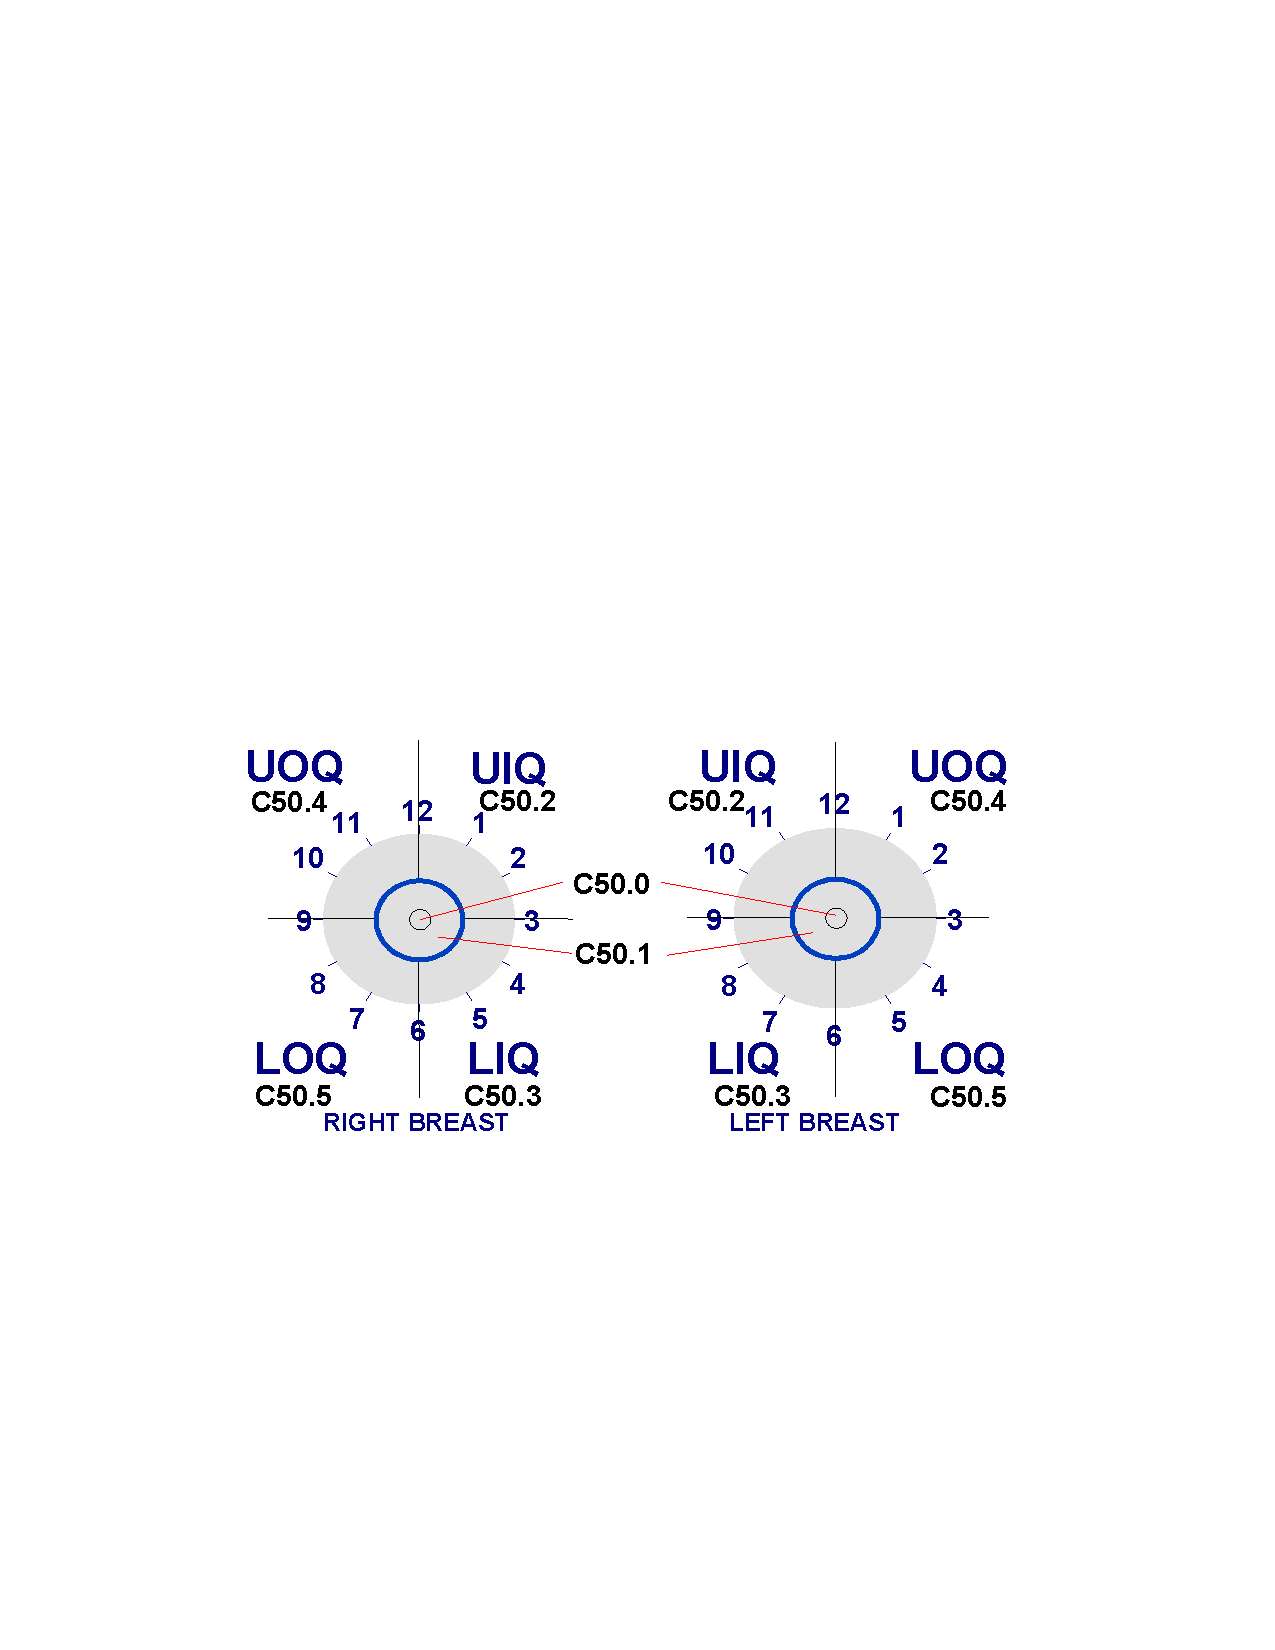
\includegraphics[width=1
	\linewidth]{IMAGENES/BREAST_CLOCK_POSITION}
	\caption{Posiciones del reloj y códigos de los cuadrantes de los senos.}
	\label{Breast_Clock}
\end{figure}

En consecuencia, de  realizar el filtrado del conjunto total de datos se obtuvo un conjunto de datos resultante de $8927$ registros. Teniendo en cuenta en nuevo conjunto de datos se generaron las gráficas que puede observarse en la figura \ref{EDA}. Dados los resultados obtenidos, se determina que  el código de diagnostico de cáncer de mama con mas numero de muertes asociadas fue el $C509$, seguido por el $C504$ respectivamente. 

\begin{figure}[h!]
	\centering
	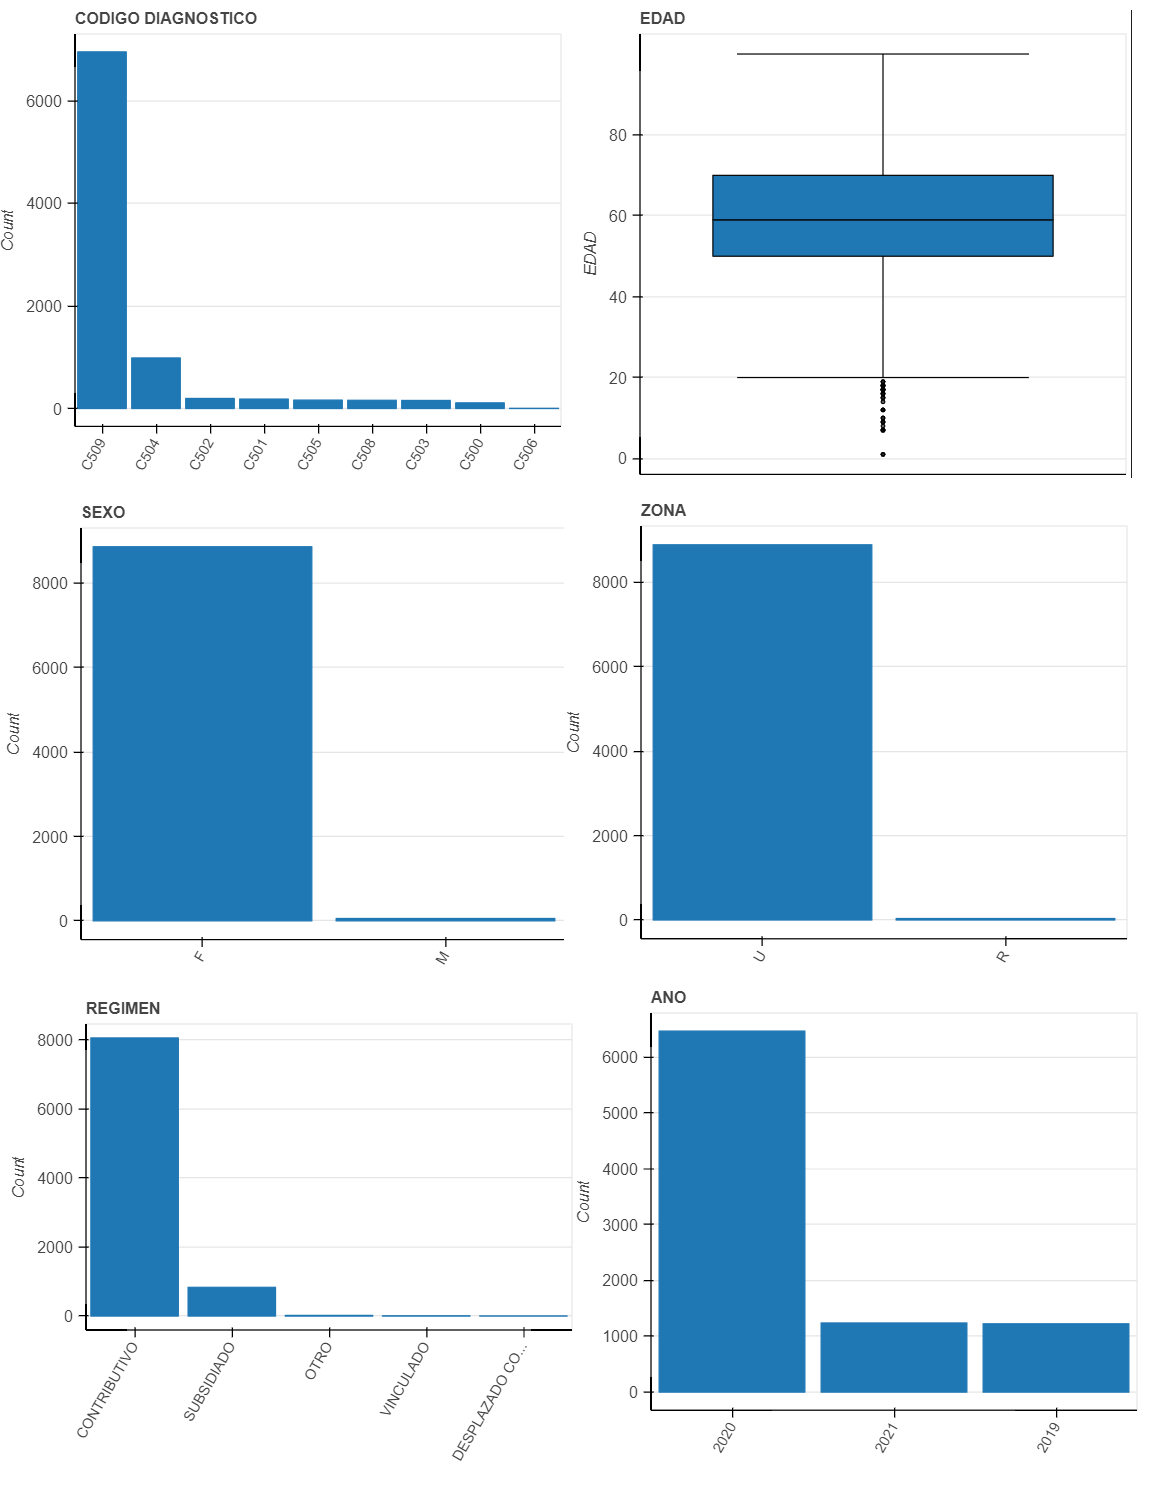
\includegraphics[width=1 
	\linewidth]{IMAGENES/EDA_BREAST}
	\caption{Diagramas analíticos cáncer de Seno C500 - C509.}
	\label{EDA}
\end{figure}

\newpage 
De igual modo, es plausible afirmar que el conjunto de datos presenta 5 variables de tipo \textit{categórica} y 2 de tipo \textit{numérica}. Adicionalmente, según los resultados obtenidos en la figura \ref{EDA}, se determina que el genero femenino entre los 50 y 70 años de edad, que habitan en zonas urbanas y que tienen una vinculación de salud de régimen contributivo presentan un mayor numero de morbilidad por cáncer de mama. Por otro lado se infiere, que en el año 2020 se presento una tasa mayor de muertes con respecto a los años 2018 y 2021.


\subsection{Fase 3: Limpieza y pre-procesamiento de datos}
En esta etapa se realizó la limpieza y el pre-procesamiento de los datos de destino para completarlos y hacerlos consistentes sin ningún tipo de ruido. Como se puede ver en la figura \ref{missing_data} la homogeneidad del conjunto de datos utilizado no generó valores perdidos, esto se debe a que fueron estandarizados por la secretaria de salud de la alcaldía municipal de Pereira.

\begin{figure}[h!]
	\centering
	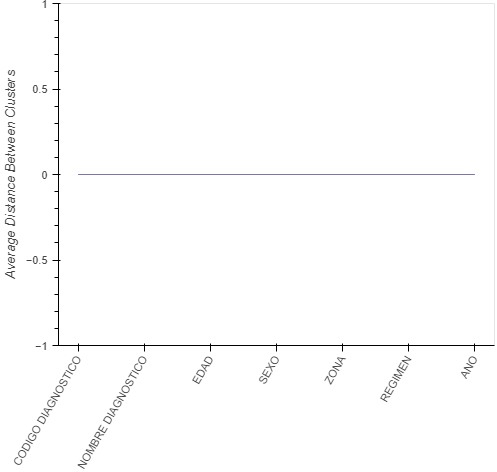
\includegraphics[width=0.9
	\linewidth]{IMAGENES/MISSING_DATA}
	\caption{Valores faltantes en el conjunto de datos.}
	\label{missing_data}
\end{figure} 



\subsection*{Fase 4: Transformación de datos}
En esta etapa se realizó la transformación de los datos para que los algoritmos en la fase de minería de datos se aplicaran fácilmente. Dado lo anterior, se detecto que los registros asociados a la variable \textit{AÑO} presentaban los valores anómalos $2.019$, $2020.000$ y  $2.02$. Dichos valores fueron reemplazados por $2019$, $2020$ y $2021$ respectivamente. De manera similar, la variable \textit{REGIMEN} presentaba registros con el texto \textit{"DESPLAZADO CON AFILIACION AL REGIMEN SUBSIDIADO"}, por lo tanto estos registros fueron reemplazados por la categoría \textit{SUBSIDIADO}. Por otra parte, se detecto que la variable categórica \textit{NOMBRE DIAGNOSTICO} presentaba una longitud que fue considerada como innecesaria para realizar el proceso de análisis los datos, puesto que por medio de la variable \textit{CODIGO DIAGNOSTICO}, según los códigos topográficos de especificados por la SEER, se puede obtener la descripción de la clasificación de los tumores múltiples causados por cáncer de mama. Por consiguiente, la variable mencionada fue eliminada del conjunto de datos. 
\subsection*{Fase 5: Minería de datos}
En esta etapa se utilizo el algoritmo \textit{k-means}, el cual hace parte del tipo de aprendizaje no supervisado, y es una de las técnicas de clustering \footnote{agrupamiento} más utilizada por su sencillez y rapidez. En este modelo, se dividen los datos en \textit{k-clusters} asignando cada objeto a su centroide de cluster más cercano (el valor medio de las variables para todos los objetos en ese cluster en particular) basado en la medida de la distancia utilizada. Es más robusto ante diferentes tipos de variables. Además, es rápido para grandes conjuntos de datos, que son habituales en la segmentación \cite{Dean2014}. El algoritmo \textit{k-means} presenta los siguientes pasos:

\begin{enumerate}
	\item Elegir el número de \textit{k-clusters}.
	\item Seleccionar \textit{k-centros} del clúster. Para ello, se debe elegir al azar \textit{k} objetos del conjunto de datos.
	\item Asignar cada objeto al centroide de cluster más cercano.
	\item Re-calcular el nuevo centroide del clúster.
	\item Repetir los pasos 3 y 4 hasta que se cumpla el criterio de convergencia o se alcance la máxima iteración.
\end{enumerate}

Cabe resaltar, que este algoritmo fue seleccionado en función de los objetivos particulares definidos en la fase 1. Para ejecutarlo, se utilizo el lenguaje multi-paradigma \textit{Python} debido a la gran cantidad librerías que permiten agilizar el entrenamiento de algoritmos de aprendizaje no supervisado. En este caso se realizó un análisis con base al agrupamiento de la totalidad de datos conformado por $8481$ filas y $6$ columnas. 

\begin{figure}[h!]
	\centering
	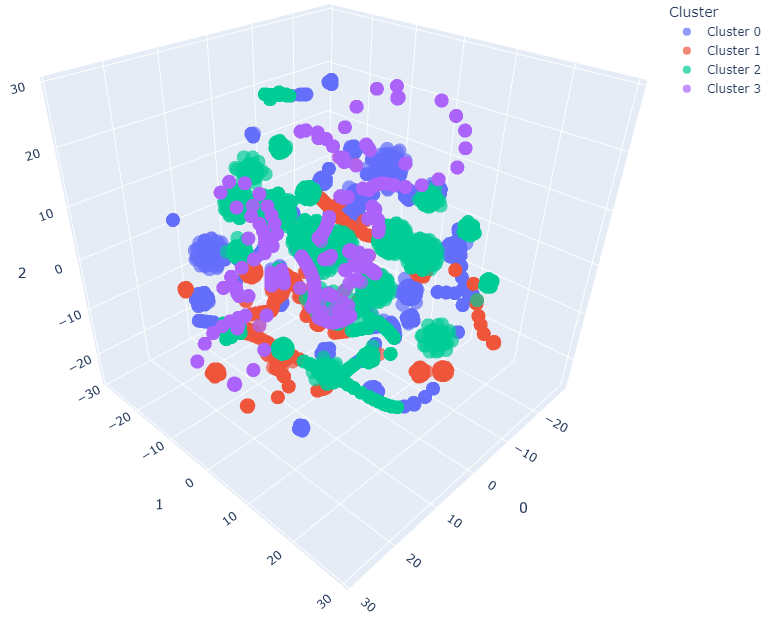
\includegraphics[width=1
	\linewidth]{IMAGENES/Tsne}
	\caption{Gráfica T-SNE para clusters.}
	\label{TSNE}
\end{figure} 

A continuación se le asigno a la creación del modelo una tolerancia del $0.0001$ con la cual le tomo un máximo de 300 iteraciones para obtener un totalidad de 4 clusters. El resultado puede ser observado en la figura \ref{TSNE}, la cual fue generada con el método T-SNE \footnote{T-distributed Stochastic Neighbor Embedding}, el cual permite generar una distribución de probabilidad que representa las similitudes entre vecinos en un espacio de gran dimensión y en un espacio de menor dimensión. Para un mejor entendimiento del resultado obtenido, en la figura \ref{Distance} se observa la distancia entre clusters con respecto a la posición inicial generada por el modelo.

\begin{figure}[h!]
	\centering
	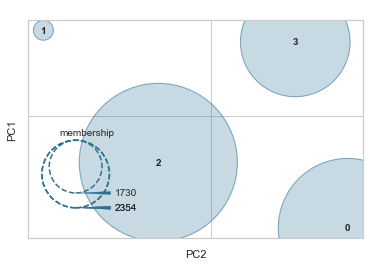
\includegraphics[width=1
	\linewidth]{IMAGENES/Distance}
	\caption{Mapas de distancia entre clusters.}
	\label{Distance}
\end{figure} 

Cabe resaltar, que para la creación, entrenamiento y prueba del modelo se utilizo una maquina equipada con un procesador Intel Core i7-11370H de 11th generación con una frecuencia de 3.30 GHz-4.9 GHz , una tarjeta NVIDIA GeForce RTX 3050, un disco duro SSD Samsung con una velocidad de lectura de  7,000 MB/s y 48GB de memoria RAM. 

Simultáneamente para demostrar el comportamiento predictivo del modelo se utilizo el $95\%$ de los datos para el entrenamiento y el $5\%$ de datos restante para comprobar la precisión en la predicción del agrupamiento con un conjunto de datos nuevo en caso de que se requiere este tipo de análisis.
\subsection*{Fase 6: Evaluación e interpretación}

En esta etapa se realizó la la evaluación e interpretación de los resultados obtenidos por el modelo \textit{k-means} visto en la fase anterior. Para ello, se utilizo el \textit{método del codo} y el \textit{método de la silueta} para determinar si el número de clusters generado por el modelo fue el adecuado. Podemos definir el coeficiente de la silueta como:

\begin{itemize}[label=]
	\item $a(x)=$ distancia promedio de $x$ a todos los demás puntos en el mismo cluster.\\
	\item $b(x)=$ distancia promedio de $x$ a todos los demás puntos en el cluster más cercano.
\end{itemize}

Dado esto, se dice que el coeficiente de la silueta para $x$ está dado por:

\begin{equation}
	s(x) = \frac{b(x)-a(x)}{max\left\lbrace a(x), b(x) \right\rbrace }
\end{equation}

\break
Donde el valor de $s(x)$ puede variar entre $-1$ y $1$. En donde, $-1$ es interpretado como un mal agrupamiento, $0$ como un resultado indiferente y $1$ como un buen agrupamiento \cite{Ramirez2018}. Por lo tanto, el coeficiente de la silueta para todo el agrupamiento es:

\begin{equation}
	SC = \frac{1}{N} \sum_{i = 1}^{N}s(x)
\end{equation}

En el caso del modelo \text{k-means} creado anteriormente, se obtuvo un valor de $k = 4$. Este valor fue comprobado por el método de la silueta obteniendo el resultado que se observa en la figura \ref{Silhouette}. En ella se puede observar que existen $4$ clusters cercanos a $1$ lo cual indica que el agrupamiento es aceptable. 

\begin{figure}[h!]
	\centering
	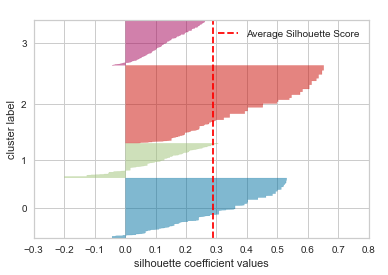
\includegraphics[width=1
	\linewidth]{IMAGENES/Silhouette}
	\caption{Método de la silueta para el modelo k-means.}
	\label{Silhouette}
\end{figure} 

Algo similar sucede con el \textit{método del codo}, el cual utiliza los valores de la inercia obtenidos tras aplicar el método \textit{k-means} a diferente número de clusters (desde $1$ a $N$ clusters), siendo la inercia la suma de las distancias al cuadrado de cada objeto del cluster a su centroide:

\begin{equation}
	inercia = \sum_{i = 0}^{N}  \parallel x_{i} - \mu  \parallel
\end{equation}

Una vez obtenidos los valores de la inercia tras aplicar el $k-means$ de $1$ a $N$ clusters, se representa en una gráfica lineal la inercia respecto del número de clusters. En esta gráfica se debería de apreciar un cambio brusco en la evolución de la inercia, teniendo la línea representada una forma similar a la de un brazo y su codo. El punto en el que se observa ese cambio nos indica el número óptimo de clusters a seleccionar para el conjunto de datos en cuestión \cite{Moya2022}. Dado lo anterior, en la figura \ref{Elbow} se observa que la inercia se produce en $k = 5 $ , lo cual indica que el modelo \textit{k-means} en cuestión tiene el numero de clusters adecuado. 

\begin{figure}[h!]
	\centering
	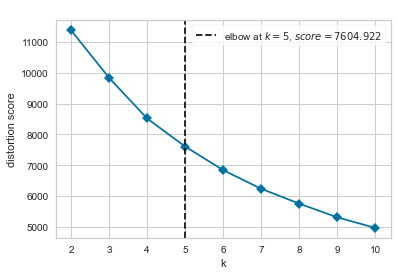
\includegraphics[width=1
	\linewidth]{IMAGENES/Elbow}
	\caption{Método del codo para el modelo k-means.}
	\label{Elbow}
\end{figure} 

Llegado a este punto, en la figura \ref{distribucion_total} se observa el la distribución obtenida para cada una de las variables en los 4 grupos generados en por el modelo \textit{k-means}, con base al conjunto de datos de morbilidad por cáncer de mama en el municipio de Pereira-Risaralda.

\begin{figure}[h!]
	\centering
	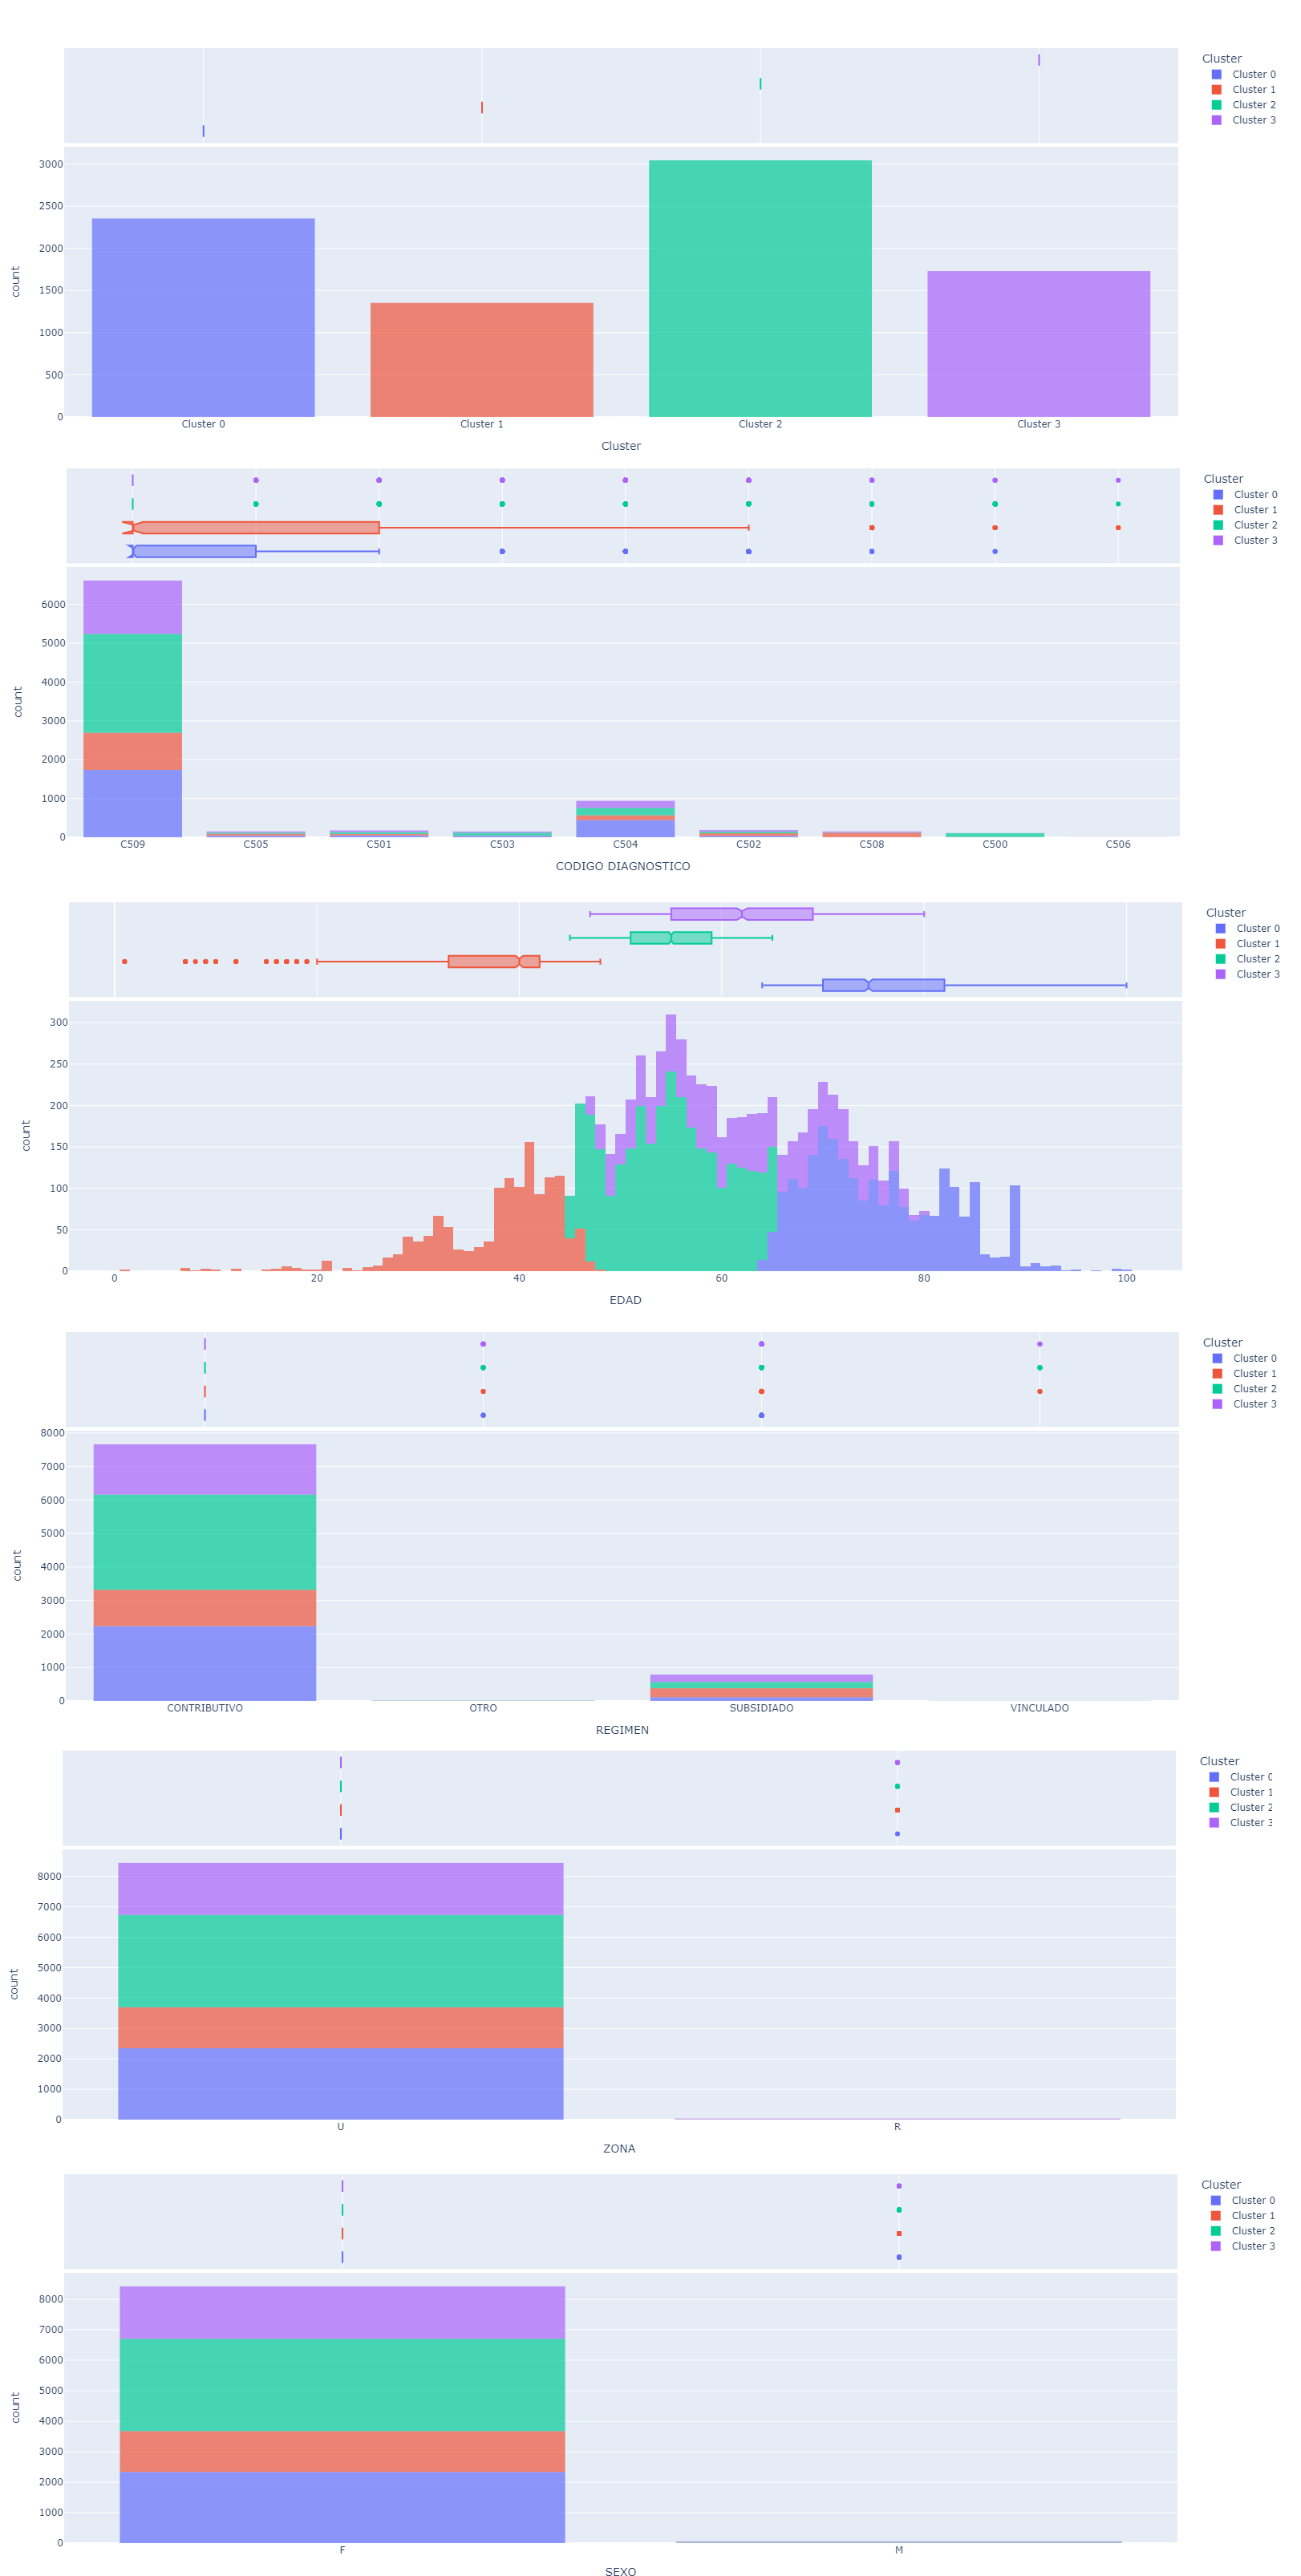
\includegraphics[width=1
	\linewidth]{IMAGENES/Distribucion_Total}
	\caption{Distribución en 4 clusters de 8481 registros.}
	\label{distribucion_total}
\end{figure} 

Interpretando los resultados obtenidos, es posible afirmar que el cáncer con código topográfico de $C509$ relacionado con múltiples tumores en diferentes sub-sitios dentro de la mama, esta presente en todos los grupos generados por el modelo \textit{k-means}. De igual forma, los sujetos de genero femenino que están afiliados a un régimen de salud contributivo y que habitan en zonas urbanas también están presentes en cada uno de los clusters. Sin embargo, aunque esta información se determino en el \textit{análisis exploratorio de datos} de la fase 1, se encontró un patrón interesante en la variable edad. Como se puede observar en la figura \ref{distribucion_total}, la morbilidad por cáncer de mama puede ser determinada como: Severa para edades entre 51 y 59 años, alta para edades entre 70 y 82 años, media para edades entre 55 y 69 años y baja para edades entre 33 y 42 años. De estos resultados es posible inferir que el cáncer de mama no presenta un comportamiento directamente dependiente con la variable edad, es decir no necesariamente la morbilidad por esta enfermedad se desarrolla en la medida en que las mujeres envejecen, por el contrario presenta su punto de letalidad mas alto en las mujeres risaraldenses con 55 años de edad. Adicionalmente, aunque el tipo de cáncer con código topográfico de $C504$ relacionado al Cuadrante superior externo (UOQ) de la mama, no estuvo contenido en ninguno de los cluster generados por el modelo se puede determinar que presento un numero de muertes significativas para mujeres con rango de edad 70 y los 82 años edad.


\section{RESULTADOS}

De acuerdo a la información generada por el modelo \textit{k-means}, se demuestra que el cáncer con código de diagnostico $C509$  presenta un mayor numero de muertes para los individuos con genero femenino que habitan en zonas urbanas, que presentan un régimen de salud contributivo y tienen una edad que oscila entre los 51 y 59 años. Complementado lo anterior, todos los clusters presentan una similitud en las variables sexo, régimen y zona, sin embargo en la variable edad el número de muertes cambia significativamente en los clusters 0,1, y 3, siendo el cluster 1 el que presenta una mortalidad menor para las mujeres con edades entre 33 y 42 años. Adicionalmente, los individuos que habitan en zonas rurales presentan un indice de muertes menor que los que habitan en zonas urbanas. De forma similar, los individuos que están afiliados al régimen subsidiado, presentan un indice de muertes menor en comparación a los que tienen una afiliación por régimen contributivo. Dado lo anterior, es posible afirmar que el cáncer de mama presenta indices mas altos de muertes en muestras de la población de Pereira-Risaralda caracterizada según su edad, genero, zona y régimen de salud, dando respuesta a la pregunta planteada para la investigación.

\section{CONCLUSIONES}
Como conclusión, es plausible afirmar que los centros especializados en ciencias de la salud y protección social enfocados en los casos cáncer de mama presentados en la población del municipio de Pereira, deben dar atención de forma urgente a las mujeres que se encuentran entre los 51 y 59 años de edad. Dado lo anterior, es necesario recalcar que como el promedio del tiempo de espera de un paciente es de 90 días desde la aparición de los síntomas hasta el diagnóstico del cáncer, la diferencia de años entre los pacientes es un factor determinante para combatir esta enfermedad. Adicionalmente, dado que la mayoría de individuos fallecidos presentaban un régimen de salud contributivo es posible inferir que la cobertura de los centros oncológicos en zonas urbanas no fue suficiente para atender todos los casos reportados de cáncer con código de diagnostico $C509$, por lo que se recomienda que cuando la coyuntura de casos presentados en los rangos de edad expuestos anterior sea muy alta, dichos casos sean remitidos de forma urgente a otros centros médicos cercanos a la ciudad de Pereira. También cabe señalar, que el tipo cáncer de mama con código de diagnostico $C504$ presento un rango de propagación menor en la mama para las mujeres entre los 70 y los 82 años edad. Este factor es importante, ya que abre paso a analizar mas a fondo que componentes celulares que forman los tejidos grasos y fibrosos de la mama son diferentes para mujeres entre los 51 y 59 años de edad, esto con el proposito de retardar el crecimiento anormal de las células cancerosas. Por ultimo, el modelo \textit{k-means} generado puede ser utilizado para determinar en que grupo se encuentra una persona que presenta variables similares a las vistas en lo largo de esta investigación, por consiguiente es posible proponer una estrategia de análisis previo para agilizar un tratamiento preventivo y así evitar que las cifras de muerte producidas por cáncer de mama aumente en la ciudad de Pereira-Risaralda.
